\documentclass[12pt,notitlepage,oneside]{report}
\setcounter{secnumdepth}{3}
\usepackage{buet_msc_thesis}
\usepackage{lipsum}
\usepackage{sectsty}
\chapternumberfont{\fontsize{16}{15}\selectfont}
\chaptertitlefont{\fontsize{16}{15}\selectfont}
\sectionfont{\fontsize{14}{15}\selectfont}
\subsectionfont{\fontsize{12}{15}\selectfont}
%\usepackage[acronym, toc]{glossaries}

% Uncomment any of the following lines should you need to
% suppress the LOF, or LOT or LOA

% \suppresslistoffigures 
% \suppresslistoftables
% \suppresslistofalgorithms

% For index creation, comment this out if you do not want to create an
% index
\makeindex[intoc]
\patchcmd{\titlepage}{empty}{fancy}{}{}
\patchcmd{\chapter}{plain}{fancy}{}{}
\begin{document}


% Edit as needed below this line
% %%%%%%%%%%%%%%%%%%%%%%%%%%%%%%%%%%%%%%%%%%%%%%%%%%%%%%%%
% Chapter-1

\chapter{Introduction}\label{intro}
 At present there are millions of sites, applications, blogs that deal with text data. Most of the data deals with complex emotions of the people. Sometimes it is about a bad product, sometimes it is simply about someone's mental health condition. In order to sort all the data and make sense of it, a system is necessary.And it is not possible for a human being to make sense of millions and billions of data. So different language processing methods was created. Methods that can give results after processing thousands of data. These methods include models like RNN, LSTM, NLP.

Long short term memory or for short, LSTM is type of recurrent neural network. It is more like a modified version which can easily remember past data in memory. LSTM uses back propagation to train itself. So the solution we discuss is to implement LSTM to detect emotions more accurately from texts using better computation methods. 

\section{Problem Statement}
The problem is that we have huge data and not enough ways to process it and get a intended outcome. Existing models don't always give accurate results on the emotion the textual data is expressing. It can easily be identified by a human but it needs to be done by machines or simply computers more efficiently using less resources while computing the result. Because a lot of the existing methods rely on heavy computational resources. By using LSTM and modifying to give better output. 

We implement emotion detection and train it with datasets from kaggle which contains data consisting of mainly four emotions. Deep learning methods has been utilised for sentence analysis and processing of emotional data. Various approaches exist today for detecting emotion from text but often it is only limited to three categories, positive, negative and neutral. Deep learning technique provides the ability to classify different emotions as well from text data.
\section{Problem Background}
Neural networks plays an important role in the world of deep learning. There are a lot of neural network models which are used for this purpose. But ass discussed earlier, not all of them provides efficient results. For example, CNN can also be used to identify emotions from texts but it has a drawback, it doesn't store the trained knowledge for it to be used later. The network needs to be trained every time we want to run tests. It starts from scratch again. That's why older neural network models cant utilize the benefit of memory storage. That's why we have deep learning capable algorithms such as LSTM, BI-LSTM which learns each and every word from the given sentences present in the corpus.   

\section{Motivations}

We are currently seeing a boom in social media popularity and ecommerce sites. More than half of the world uses social media for different interactions and a quarter of the people now prefer ecommerce sites for purchases of different necessities. The use of texts in these sites is seen excessively as people share their opinions as posts, blogs and reviews in social media and reviews of products in different ecommerce sites. As a result, we now have a very big resource in our hand which can be used for providing tailor made services for the customers by service providers. Determining emotion from texts can help us reach a verdict on a topic or a product from thousands or millions of people. It will be possible to determine whether a service is appreciated or hated by the people simply from their posts, reviews in an instant, saving tons of time and playing a big role in product improvement. Furthermore, it can be also applied in applications such as emotion retrieval from suicide notes, detecting insulting sentences in chat conversations and so on. Therefore, a better method of detecting emotion from text based data is very crucial in the modern world.

\section{Research Objectives}
There are many emotion detection techniques but not all of them provide state of
the art accuracy. There are abundant ways to make it more efficient and less time
consuming on the hardware capability end. The objectives of this project include –
\begin{itemize}
\item To better understand the concept of LSTM model and its word embedding techniques
\item To improve accuracy of emotion detection from texts using LSTM model
\item To detect wide range of emotions from given text in terms of anger, fear, joy and sadness 
\item To build a better algorithm to be implemented in applications like sentiment analysis
\end{itemize}

\section{Significance of the Research} 
Emotion detection allows the ability to extract insights from comments on social media, survey data or other sources of feedback methods. These insights are often helpful in understanding targeted people's perspective. It can also be used to determine mental condition of suicidal patients from their diaries or blogs. Which is why emotion detection is greatly important in this digital era. Therefore accurate results from such research will be of great importance to the world. 

\section{Key Contribution}
This research offers its contribution in improving accuracy of LSTM by fine tuning its architecture, improving performance with data training and optimizing it to have better learning rate and proper weight initialization.

% Chapter-2
\chapter{Background Study} \label{ch:literature_review}


Emotions that incite individuals to write down certain words at particular times are what emotion detection is about. People often convey their feelings through texts, words. That's why it has been the topic of research for many. Researchers often try to create or innovate or perfect systems to better understand how emotions can be extracted in a meaningful way. Deep learning has also paved the way for researchers to further study this topic.
\section{Literature Review}

\subsection{Emotion Correlation Mining Through Deep Learning Models on Natural Language Text}
Xinzhi Wang et al.[1] introduced an embedded recursive neural network for improving emotion recognition, Long Short-Term Memory (LSTM) was used as a variant of RNNs. This method determines to do the potential and meaningful correlation among emotions from Web news. Tow deep neural network models, CNN-LSTM2 and CNN-LSTM-STACK are employed for emotion recognition. The data sets are collected from one of the most popular social platforms, news channel. Emotion correlation differs for different types datasets. In objective texts, some emotions be misinterpreted as love. Also, emotions are easily mistaken as anger. Yet, it achieved greater than 85\% and approaches 90\%.


\subsection{Topic-Enhanced Capsule Network for Multi-Label Emotion Classification}
Donghong Ji et al.[2] developed a capsule network which is effectively leveraging for multiple emotion prediction. This model consists of two components, a topic module and a capsule model. The topic module takes Bag of Words (BoW) as input via Variational Autoencoder (VAE) and learns latent topics and keywords. Then the capsule module captures encapsulated features for each emotion from low level to high level via three deep capsule layers. In the learning process, they pre-train the emotion module and co-train the entire part with a batch size of 16, both under early-stop strategy. Results on the benchmark data-sets showed that their method outperformed strong baselines by a large margin.



\subsection{An Experimental Analysis of Data Annotation Methodologies for Emotion Detection in Short Text Posted on Social Media}

Maria Krommyda et al.[3] proposed a hybrid rule-based algorithm that allows the acquisition of a dataset that is annotated with regard to the Plutchik's eight basic emotions. This technique is not focusing on the positive or negative opinions expressed but tries to determines the human emotion that is expressed. A total of 1.2 million annotated tweets were downloaded. Eighty percent of them were used as a training sample, 10\% as validation and 10\% as testing. The LSTM network was used and achieved 91.9\% accuracy. Yet, this system is weak to detect some particular emotion such as disgust and joy. But the overall performance of the system is quite significant. 


\section{Problem Analysis}








% Chapter-3
\chapter{Proposed System}
\label{ch:Proposed System}
Emotion detection from text has now become one of the key feature to understand peoples emotion. Everyone writes about their feelings or emotion in their social media, comment box or in inbox. If a system can identify those emotions from texts then it will be very help full to understand the people's thoughts. For this reason we build a system that can detect emotion from text. In this chapter we represents our architectural diagram and detailed module design of our text based emotion detection system.

\section{Design}
Here we represent the architectural design of the system. In our system we use text data from Whatsapp. We export the chat data into text file. Then we processed the data and make a suitable data formate to detect emotion. Then this data formate are sent to the finale stage where the emotion is detected using LSTM network architecture.

\begin{figure}
  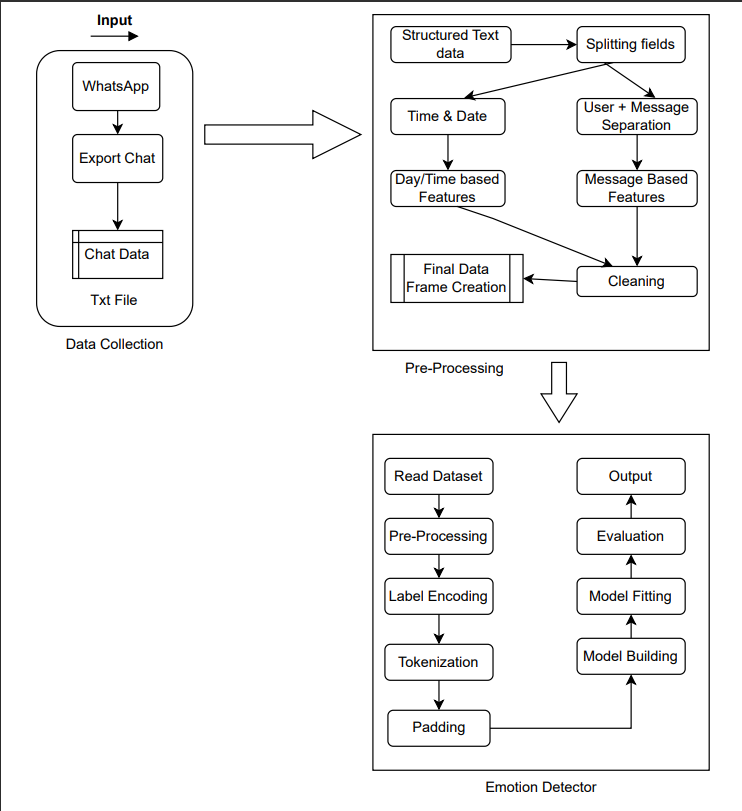
\includegraphics[width=\linewidth]{chapters/arcdesign.png}
  \caption{System architecture}
\end{figure}


\section{Module Description}
Here we provide detailed information about the modules of our system. That defines how our system works.
\begin{itemize}
\item Data collection
\item Pre-processing
\item FastText Word Vector Model
\item LSTM
\end{itemize}

\subsection{Data Collection}
To run our system at first we need a data set from where we can perform emotion detection. For our system we choose Whatsapp for our dataset. From a Whatsapp group we can easily collect our desire dataset. Whasapp export all chats in form of text file by default. It exports chats in a fixed pattern that is [Timestamp-Username-Messages]. There are also two options, we can export chats either with media or without media. Thus our system only suitable for text so we need chats without media.
 
To collect chat data from Whatsapp at first we have to open Whatsapp on phone. Then open an individual group or chat. Then click three dot from the right top corner of the screen. Here we found More option. Then click More option. After that click on Export Chat. That's how we can collect raw dataset.

\subsection{Pre-processing}
After export the chats we load it into the application to do this at first we have to extract all the information like time, date, day, user, messages etc. Then we have to remove stop words and punctuations. There are some major modules in preprocessing:
\begin{itemize}
\item \textbf{Splitting Fields:} We previously mentioned that the pattern of Whatsapp data is [Timestamp-Username-Messages]. So in this step the Timestamp is extracted from the chat using regular expression.

\item \textbf{Data frame creation:} After Timestamp and message are extracted the data frame is created. TO create the data frame pandas library is used.

\item \textbf{Date format conversion:} Whatsapp is installed locally in each device. That's why the data set will be in device's date format such as [DD/MM/YYYY, DD/MMM/YY, MM/DD/YYYY, MM/DD/YY etc]. But Python date format is YYYY/MM/DD. So here the custom date format is converted into Python's date format.

\item \textbf{Time format conversion:} Time is also present in custom format in each device just like date such as 12 hour format, 24 hour format. So in this step custom date formats are converted into a single date format which is 24 hour date format.
 
\item \textbf{Feature addition:} Here other meaningful information are extracted from all fields. For example Day, Date, Hour, Minute, Day Part, Period etc. has been extracted from timestamp. Similarly URLs, emojis, word count, media count etc. are also extracted from the messages part.
 
\item \textbf{Cleaning:} Here punctuations, stop words and unnecessary data are removed. 
\end{itemize}

\subsection{FastText Word Vector Model}
In sentiment evaluation word embedding techniques are considered as an important factor. FastText is a word embedding technique which is used in our system. Fasttext model is a extended version of word2vec model. Usual embadded technique uses word to build word embedding but Fasttext works one level deeper. It uses part of the word to build word embedding. For example the word, “normal” with n=3,the fastText representation of this word is ⟨nor,orm,rma,mal⟩, where the angular brackets indicatethe beginning and end of the word.

\subsection{LSTM}
LSTM stands for long short-term memory networks which is used in the field of Deep Learning.LSTM is a advanced version of recurrent neural networks (RNNs) that is design to learn long-term dependencies, especially in sequence prediction problems.

\subsubsection{Architecture of LSTM}
The role of an LSTM model is held by a memory cell known as
a cell state that maintains its state over time. The cell state is the horizontal line that runs through the top of the below diagram. Information can be added to or removed from the cell state in LSTM and is regulated by gates. These gates optionally let the information flow in and out of the cell. It contains a point-wise multiplication operation and a sigmoid neural net layer that assist the mechanism. The sigmoid layer gives out numbers between zero and one, where
zero means nothing should be let through, and one means everything should be let through.


\begin{figure}[h!]
  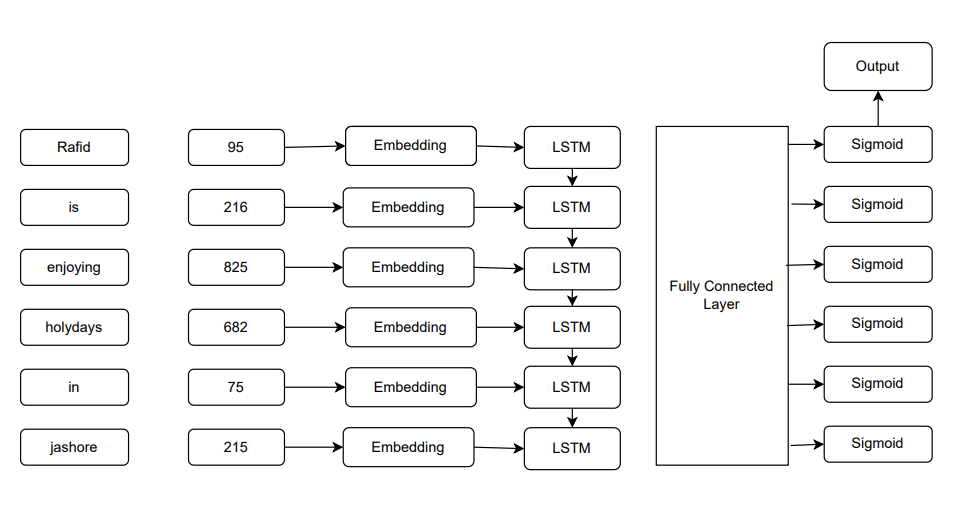
\includegraphics[width=\linewidth]{chapters/LSTM.png}
  \caption{LSTM architecture}
\end{figure}

There are mainly five layers in LSTM network. But layer an be added to improve the accuracy of the model. The five layers are:
\begin{itemize}
\item \textbf{Embedding Layer:} This Layer is responsible for converting word tokens into embedding of a specific size like 256, 512 etc. This layer maps a sequence of word indices to embedding vectors and learns the word embedding during training.
In this layer the word tokens are converted into embedding of a specific size like 256,512 etc. This layer also responsible for mapping a sequence of word indices to embedding vectors and learns the word embedding during training.

\item \textbf{LSTM Layer:}This layer sequentially process data and keep its hidden state through time. It keeps previous memory and process with current memory and decides whether to keep current memory or remain with old memory.
   
\item \textbf{Fully Connected Layer:} This layer indicates those layers where all inputs from one layer are connected to every unit of the next layer.

\item \textbf{Sigmoid Activation Layer:} This layer is responsible for converting all output values in the range of 0 to 1. It means it can either let no flow or complete flow of information throughout the gates.

\item \textbf{Output Layer:} Output layer is the final layer of the architecture. This layer is responsible for generating output which is obtained from sigmoid layer. The output formate is 2d array of real numbers where the first dimension indicates the number of samples given to the LSTM layer and second dimension is the dimensionality of the output space defined by the units
parameter in Keras LSTM implementation.
\end{itemize}
































% Chapter-4
\chapter{Proposed  System} \label{ch:methodology}
Filename: chapters/methodology.tex

In this chapter, we discuss the proposed system...  


\begin{table}
	\centering
	\caption{Example Table \label{table:summary_tn}}
	\begin{tabular*}{32pc}{@{\extracolsep{\fill}}ll@{}}
		\hline \noalign{\vspace{3pt}}
		\textbf{Hyperparameter} &\qquad \textbf{Value} \\ [3pt] \hline\noalign{\vspace{3pt}}
		Optimizer     			&\qquad Adam~\cite{Kingma_15} \\[3pt]
		Objective function  	&\qquad Fusion of softmax and center loss \\[3pt]
		Epochs        			&\qquad $ 450 $ \\ [3pt]
		Initial learning rate	&\qquad $5 \times 10^{-3}$  \\[3pt]
		Mini-batch size			&\qquad $ 256 $ \\
		\hline
	\end{tabular*}
\end{table}



% Chapter-5
\chapter{Experimental Results}\label{ch:experimental_result}
Filename: chapters/result\_discussion.tex

In this chapter, we are going to evaluate our proposed method ...

% Chapter-6
\chapter{Conclusions}\label{ch:conclusion}

\section{Conclusions}


\section{Future Prospects of Our Work}



% Chapter showing example of index creation
%\chapter{Index Creation}
\section{BUET}
Bangladesh University of Engineering and Technology, abbreviated as
BUET\index{BUET}, is one of the most prestigious institutions for
higher studies in the country. About 5500 students are pursuing
undergraduate\index{BUET!undergraduate} and
postgraduate\index{BUET!postgraduate} studies in engineering,
architecture, planning and science in this institution. At present,
BUET has sixteen teaching departments under five faculties and it has
three institutes. Every year the intake of undergraduate students is
around 900, while the intake of graduate students in Master's and PhD
programs is around 1000. A total of about five hundred teachers are
teaching in these departments and institutes. There are additional
teaching posts like Dr.\ Rashid Professor, Professor Emeritus and
Supernumerary Professors.
 
\section{Campus}
The BUET campus is in the heart of Dhaka\index{Dhaka} --- the capital
city of Bangladesh. It has a compact campus with halls of residence
within walking distances of the academic buildings. The physical
expansion of the University over the last three decades has been
impressive with construction of new academic buildings,
auditorium\index{BUET!auditorium} complex, halls of residence, etc.
 
\section{History}\index{BUET!History}
BUET is the oldest institution for the study of Engineering and
Architecture in Bangladesh. The history of this institution dates back
to the days of Dhaka Survey School which was established at
Nalgola\index{Nalgola}, in Old Dhaka in 1876 to train Surveyors for
the then Government of Bengal of British India. As the years passed,
the Survey School became the Ahsanullah School of
Engineering\index{Ahsanullah School of Engineering} offering
three-year diploma courses in Civil, Electrical and Mechanical
Engineering. In recognition of the generous financial contribution
from the then Nawab of Dhaka, it was named after his father Khawja
Ahsanullah. It moved to its present premises in 1912. In 1947, the
School was upgraded to Ahsanullah Engineering College as a Faculty of
Engineering under the University of Dhaka, offering four-year
bachelor’s courses in Civil, Electrical, Mechanical, Chemical and
Metallurgical Engineering. In order to create facilities for
postgraduate studies and research, Ahsanullah Engineering College was
upgraded to the status of a University in 1962 and was named East
Pakistan University of Engineering and Technology. After the War of
Liberation in 1971\index{1971|see {War of Liberation}}\index{War of
  Liberation}, Bangladesh became an independent state and the
university was renamed as the Bangladesh University of Engineering and
Technology.
 
\section{Students}
Till today, it has produced around 25,000 graduates in different
branches of engineering and architecture, and has established a good
reputation all over the world for the quality of its graduates, many
of whom have excelled in their profession in different parts of the
globe. It was able to attract students from countries like
India\index{India}, Nepal\index{Nepal}, Iran\index{Iran},
Jordan\index{Jordan}, Malaysia\index{Malaysia}, Sri Lanka\index{Sri
  Lanka}, Pakistan\index{Pakistan} and Palestine\index{Palestine}.
 
\section{Departments}
Both Undergraduate and Postgraduate studies and research are now among
the primary functions of the University. Eleven departments under five
faculties offer Bachelor Degrees, while most of the departments and
institutes offer Master's Degrees and some of the departments have
Ph.D. programs. In addition to its own research programs, the
university undertakes research programs sponsored by outside
organizations like European Union, UNO,
Commonwealth\index{Commonwealth}, UGC\index{UGC}, etc. The expertise
of the University teachers and the laboratory facilities of the
University are also utilized to solve problems and to provide
up-to-date engineering and technological knowledge to the various
organizations of the country.


\endinput


% Bibliographies and appendices
% You do not need to change anything in this file. If you want to
% change the reference style, comment/uncomment the \bibliographystyle
% lines

\clearpage
\renewcommand\bibname{References}
\addcontentsline{toc}{chapter}{\textbf{References}}

% Comment/uncomment as suits you
 \bibliographystyle{IEEEtran} %% IEEE transaction style
% \bibliographystyle{acm} %% ACM style
% \bibliographystyle{alpha}


\bibliography{buet_msc_thesis.bib}
%\addbibresource{buet_msc_thesis.bib}
\endinput


% Index, comment this out if you do not want to create an index
\printindex

\appendix
% Algorithms
%\input{chapters/algorithms.tex}

\end{document}